%%%%%%%%%%%%%%%%%%%%%%%%%%%%%%%%%%%%%%%%%%%%%%%%%%%%%%%%%%%%%%%%%%
%%%%%%%% ICML 2013 EXAMPLE LATEX SUBMISSION FILE %%%%%%%%%%%%%%%%%
%%%%%%%%%%%%%%%%%%%%%%%%%%%%%%%%%%%%%%%%%%%%%%%%%%%%%%%%%%%%%%%%%%

% Use the following line _only_ if you're still using LaTeX 2.09.
%\documentstyle[icml2013,epsf,natbib]{article}
% If you rely on Latex2e packages, like most moden people use this:
\documentclass{article}

% For figures
\usepackage{graphicx} % more modern
%\usepackage{epsfig} % less modern
\usepackage{subfigure} 
\usepackage{mathptmx}
%\usepackage{times}
\usepackage{microtype}
\usepackage{mdwlist}
\usepackage{bm}
\usepackage{multirow}

% For citations
\usepackage{natbib}
%\setlength{\bibsep}{0.053in}
%\renewcommand{\baselinestretch}{0.985}
%\usepackage[hang,flushmargin]{footmisc} 

% For algorithms
\usepackage{algorithm}
\usepackage{algorithmic}

\usepackage{amsmath}
\usepackage{amssymb}
\usepackage{latexsym}
\usepackage{sectsty}
\usepackage{amsfonts}

% As of 2011, we use the hyperref package to produce hyperlinks in the
% resulting PDF.  If this breaks your system, please commend out the
% following usepackage line and replace \usepackage{icml2013} with
% \usepackage[nohyperref]{icml2013} above.
\usepackage{hyperref}

% Packages hyperref and algorithmic misbehave sometimes.  We can fix
% this with the following command.
\newcommand{\theHalgorithm}{\arabic{algorithm}}

% \ref conveniences

\newcommand{\mysec}[1]{Section~\ref{sec:#1}}
\newcommand{\myapp}[1]{Appendix~\ref{app:#1}}
\newcommand{\myeq}[1]{Eq.~\ref{eq:#1}}
\newcommand{\myeqp}[1]{Eq.~\ref{eq:#1}}
\newcommand{\mychap}[1]{Chapter~\ref{chap:#1}}
\newcommand{\myfig}[1]{Figure~\ref{fig:#1}}

% math conveniences

\newcommand{\df}{{\rm d}}
\newcommand{\g}{\,\vert\,}
\newcommand{\E}{\textrm{E}}
\newcommand{\vct}[1]{\textbf{#1}}
\newcommand{\realline}{\mathbb{R}}
\newcommand{\indpt}{\protect\mathpalette{\protect\independenT}{\perp}}
\def\independenT#1#2{\mathrel{\rlap{$#1#2$}\mkern2mu{#1#2}}}
\newcommand{\h}[1]{\textrm{H}\left( #1 \right)}
\newcommand{\half}{\frac{1}{2}}
\newcommand{\new}{\textrm{new}}

\newcommand{\mult}{\textrm{Mult}}
\newcommand{\dir}{\textrm{Dir}}
\newcommand{\discrete}{\textrm{Discrete}}
\newcommand{\Bern}{\textrm{Bern}}
\newcommand{\DP}{\textrm{DP}}
\newcommand{\GP}{\textrm{GP}}
\newcommand{\Bet}{\textrm{Beta}}
\newcommand{\expect}[2]{\mathbb{E}_{#1}\left[ #2 \right]}
\renewcommand{\algorithmicrequire}{\textbf{Input:}}
\renewcommand{\algorithmicensure}{\textbf{Output:}}


% Employ the following version of the ``usepackage'' statement for
% submitting the draft version of the paper for review.  This will set
% the note in the first column to ``Under review.  Do not distribute.''
\usepackage[]{icml2013} 
% Employ this version of the ``usepackage'' statement after the paper has
% been accepted, when creating the final version.  This will set the
% note in the first column to ``Appearing in''
%\usepackage[accepted]{icml2013}


% The \icmltitle you define below is probably too long as a header.
% Therefore, a short form for the running title is supplied here:
%\icmltitlerunning{Unsupervised Object Detection, Tracking and Appearance Learning with Dependent Dirichlet Process Mixtures}
%\icmltitlerunning{Unsupervised Object Detection, Tracking, and Appearance Learning with the DDPMoO}
\icmltitlerunning{The DDPMO for Detection-free Tracking and Object Modeling}

\begin{document}

\twocolumn[
%\icmltitle{Unsupervised Object Detection, Tracking, and Appearance Learning \\with Dependent Dirichlet Process Mixtures} 
%\icmltitle{Dependent Dirichlet Process Mixture of Objects Model \\for Unsupervised Object Detection, Tracking, and Appearance Learning} 
%\icmltitle{Unsupervised Object Detection, Tracking, and Appearance Learning \\with the Dependent Dirichlet Process Mixture of Objects Model} 
%\icmltitle{Detection-free Tracking and Appearance Learning with \\the Dependent Dirichlet Process Mixture of Objects Model} 
\icmltitle{The Dependent Dirichlet Process Mixture of Objects \\for Detection-free Tracking and Object Modeling} 

% It is OKAY to include author information, even for blind
% submissions: the style file will automatically remove it for you
% unless you've provided the [accepted] option to the icml2011
% package.
\icmlauthor{Willie Neiswanger}{willie@cs.cmu.edu}
\icmladdress{Machine Learning Dept.,
            Carnegie Mellon University,
            5000 Forbes Ave., Pittsburgh, PA, 15213, USA}
\icmlauthor{Frank Wood}{fwood@robots.ox.ac.uk}
\icmladdress{Dept. of Engineering Science, 
            Oxford University,
            Parks Road, Oxford, OX1 3PJ, UK}

% You may provide any keywords that you 
% find helpful for describing your paper; these are used to populate 
% the "keywords" metadata in the PDF but will not be shown in the document
\icmlkeywords{detection, tracking, dirichlet process, bayesian inference}

\vskip 0.3in
]

\begin{abstract}
%Many strategies for detecting and tracking objects in videos require pre-built object detectors, and suffer when the objects are unknown, their appearances vary, video quality is low, or video background is not homogeneous. 


This paper explores the question of how to find, track, and learn models of arbitrary objects in a video without a predefined method for object detection.
We present a model that localizes objects via unsupervised tracking while learning a representation of each object, avoiding the need for pre-built detectors. Our model uses a dependent Dirichlet process mixture to capture the uncertainty in number of objects and requires only spatial and color video data that can be efficiently extracted via frame differencing. We give two algorithms for performing inference and demonstrate our method on multiple videos. 
Results illustrate its ability to accurately find, track, and model diverse objects moving over non-uniform backgrounds and through occlusion. We demonstrate the model in difficult detection scenarios, on a video containing a large number of objects, and on a recent human-tracking benchmark where we show performance comparable to state of the art detector-based methods.


%Many strategies for detecting and tracking objects in videos require pre-built object detectors, and suffer when the objects are unknown, their appearances vary, video quality is low, or video background is not homogeneous. This paper explores the question of how to find, track, and learn models of arbitrary objects in a video without a predefined method for object detection.

%We present a model that localizes objects via unsupervised tracking while learning a representation of each object, avoiding the need for detectors. Our model uses a dependent Dirichlet process mixture to capture the uncertainty in number of objects and requires only spatial and color pixel data that can be efficiently extracted from videos via frame differencing. We give two algorithms for performing inference and demonstrate our method on multiple videos. Results illustrate its ability to find, track, and model diverse objects moving over non-uniform backgrounds and through occlusion. We also show results on a recent human-tracking benchmark that are comparable to state of the art detector-based methods.
\end{abstract}

\section{Introduction}
Algorithms for automated object detection and tracking in video have found application in a wide range of fields, including robotic vision, cell tracking, sports analysis, video indexing, and video surveillance \cite{turaga2008machine,yilmaz2006object}. 
The goal of these algorithms is to find the sequences of positions held by each object of interest in a video. A majority of modern methods require a pre-trained object detector or make use of prior knowledge about the objects' physical characteristics (such as their color or shape) to perform detection \cite{breitenstein2009robust}. Often, these methods will apply the detector in each frame of a video, and then use the detection results in tracking or data association algorithms. Other algorithms use heuristics to find, or require manual initialization of, object positions and then search for similar image patches in consecutive frames to perform tracking \cite{meer2003kernel}. Both techniques require some predefined detection strategy for each type of object they intend to find and track.

When the objects to be tracked have highly variable appearance, if one wishes to track many different types of objects, or if one simply does not know the types of objects in advance, it is often hard to find a suitable detection strategy \cite{babenko2011robust}. Furthermore, common video conditions such as variable lighting, low quality images, non-uniform backgrounds, and object occlusions can all reduce the accuracy of detection \cite{wu2007cluster}.

Cases such as these, where constructing an object detector may be infeasible, prompt the need for a method to automatically localize and track arbitrary objects. 
Some classic methods towards this end have involved background subtraction and blob tracking, which segment foreground patches to localize objects, and optical flow-based tracking, which separate objects based on their relative motion. Both have trouble consistently and accurately segmenting objects and tracking through occlusion \cite{veeraraghavan2006robust,barron1994performance}.
A recent work introduced the term ``detection-free tracking'' for this task, and proposed a method based on spectral clustering of trajectories \cite{fragkiadaki2011detection}.

Bayesian models have also been employed to capture the components of a video, and a number of recent works have incorporated nonparametric Bayesian priors for finding the patterns of motion in scenes \cite{wang2007unsupervised,emonet2011extracting}. However, there has been little towards building Bayesian models that model arbitrary video objects in order to perform high quality detection-free tracking.

In this paper, we develop a nonparametric Bayesian model for jointly learning a representation of each object and performing unsupervised tracking, thereby allowing for accurate localization of arbitrary objects. We combine a dependent Dirichlet process mixture with object and motion models to form the dependent Dirichlet process mixture of objects (DDPMO). The advantages of our model are that it can (a) accurately discern arbitrary video objects and track them in a fully unsupervised fashion, (b) jointly learn a model for each object and use these models to aid in object localization/tracking, (c) infer a distribution over the number of distinct objects present in a video, (d) incorporate a model for the motion of each object, and (e) begin tracking as objects enter the video frame, stop when they exit, and track through periods of partial or full occlusion.

%In Section 2 we describe data extraction and define the DDPMO, in Section 3 we present inference algorithms and discuss computational efficiency, in Section 4 we present experimental results, and we conclude in Section 5.

\section{Dependent Dirichlet Process Mixture of Objects (DDPMO)}

\subsection{Data Extraction}
Our model operates on spatial and color pixel data that can be efficiently extracted via frame differencing: in each frame t, we find the pixel values that have changed beyond some threshold, and record pixel positions $\mathbf{x}^s_{t,n} = (x^{s_1}_{t,n}, x^{s_2}_{t,n})$ (where $n=1,\ldots,N_t$ indexes the extracted pixels at time $t$). Additionally, the spectrum of RGB color values is discretized into $V$ bins, and the local color distribution around each pixel is described by counts of surrounding pixels (in an $m \times m$ grid) that fall into each color bin, denoted $\mathbf{x}^c_{t,n} = (x^{c_1}_{t,n},\ldots,x^{c_{V}}_{t,n})$. Observations are therefore of the form
\begin{equation}
    \mathbf{x}_{t,n} = (\mathbf{x}^s_{t,n},\mathbf{x}^c_{t,n}) = (x^{s_1}_{t,n},x^{s_2}_{t,n},x^{c_1}_{t,n},\ldots,x^{c_{V}}_{t,n})
\end{equation}
Examples of spatial pixel data extracted via frame differencing are shown in Figure~\ref{fig:fig01}.
\begin{figure}[h]
        \center{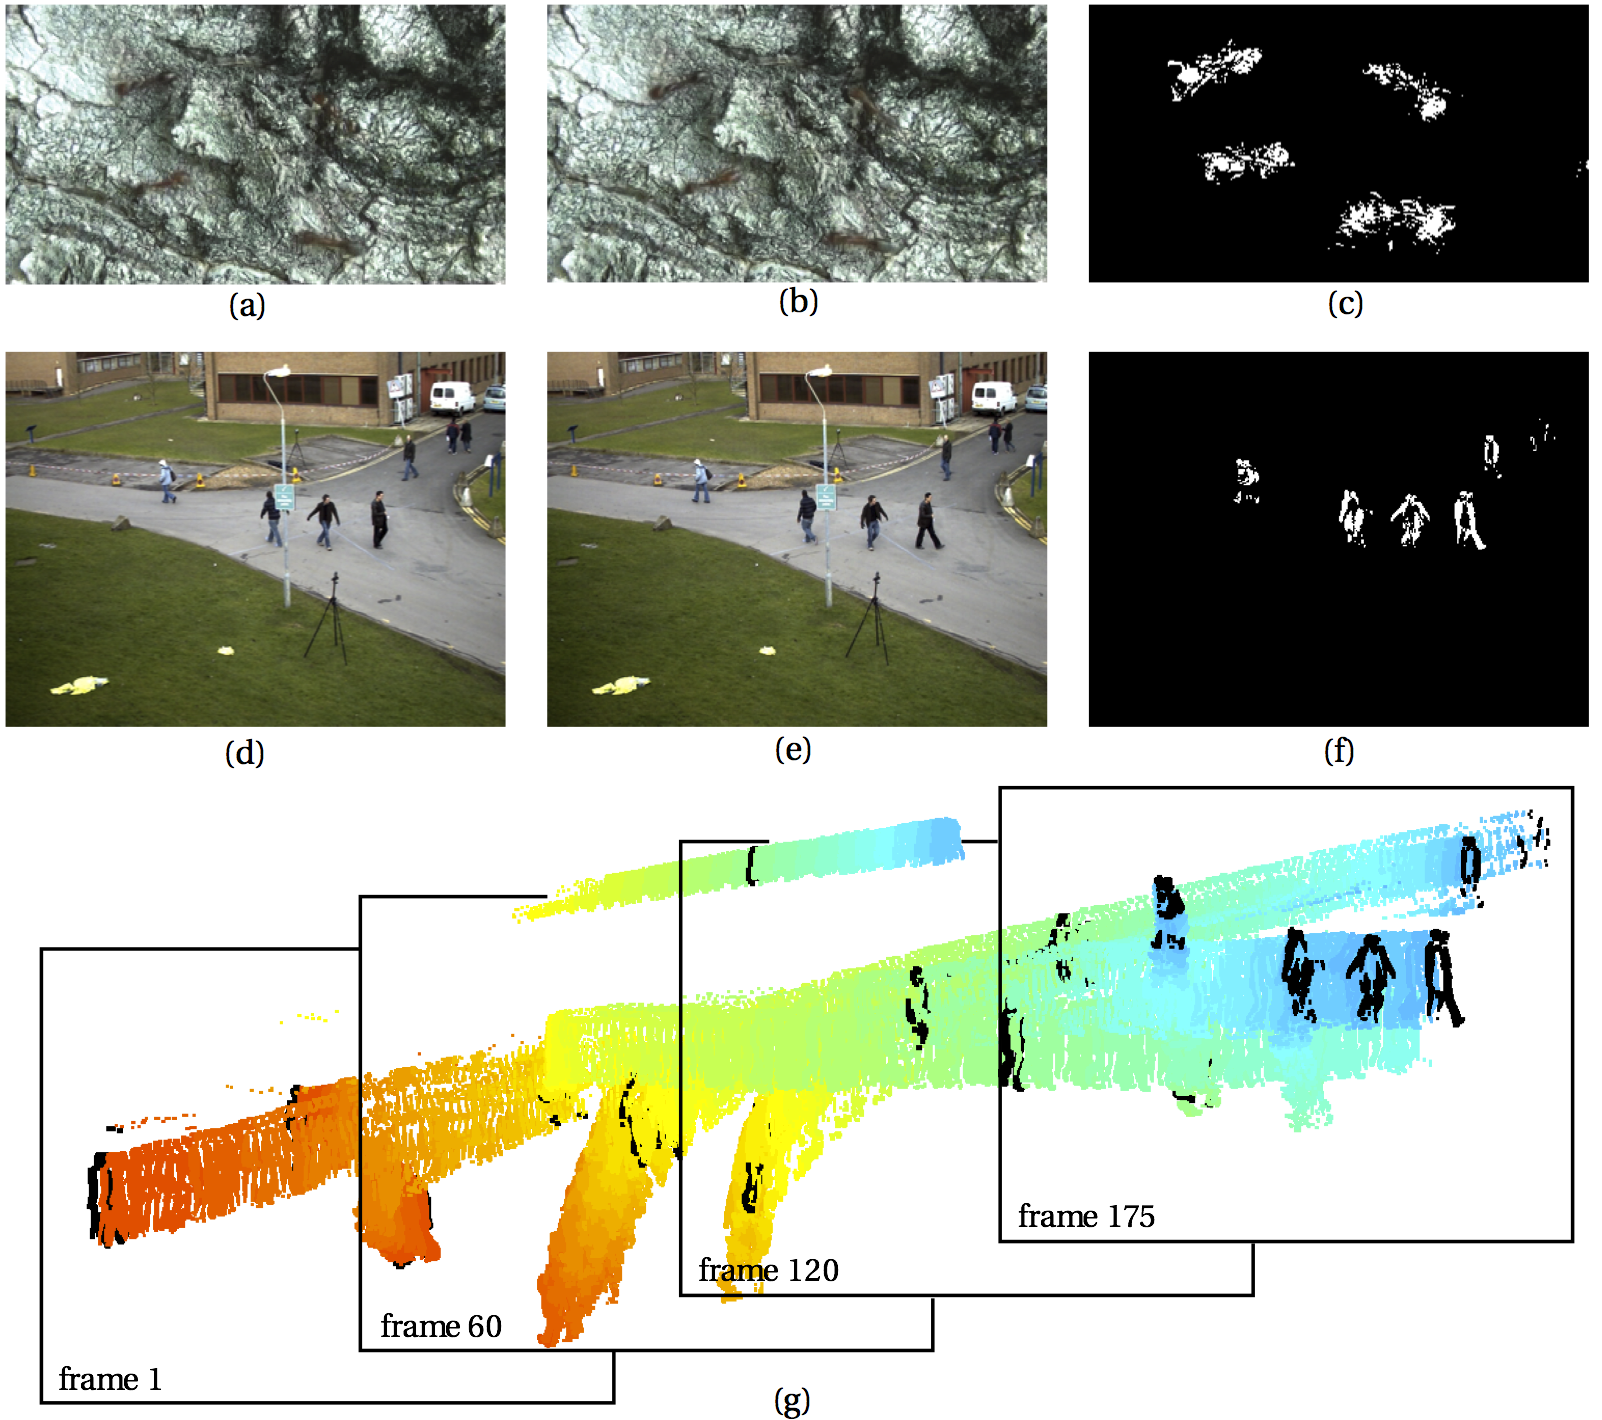
\includegraphics[width=80mm]{icml_fig01.png}}
        \caption{\label{fig:fig01} Two pairs of consecutive frames and the spatial observations $\mathbf{x}_{t,n}^s$ extracted by taking the pixel-wise frame difference between each pair (a - f). The final image shows the results of frame differencing over a sequence of images (from the PETS2010 dataset).}
\end{figure}


\subsection{Object Model}
An object model F is a distribution over observations
\begin{equation}
    \mathbf{x}_{t,n} \sim \text{F}(\theta_t^k)
\end{equation}
where $\theta_t^k$ denotes the parameters of the $k^{\text{th}}$ object at time $t$. We wish to keep our object model general enough to be applied to arbitrary video objects, but specific enough to learn a representation that can aid in tracking. In this paper, we model each object with
\begin{align}
    \mathbf{x}^s_{t,n} &\sim \text{Normal}(\mu_t,\Sigma_t)
    = \frac{e^{-\frac{1}{2}(\mathbf{x}^s_{t,n} - \mu_t)^{\top} \Sigma_t^{-1} (\mathbf{x}^s_{t,n} - \mu_t)}}
        {(2\pi)^{d/2}|\Sigma_t|^{1/2}}\\
        \mathbf{x}^c_{t,n} &\sim \text{Mult}(\delta_t)
        = \frac{m^2!}{x^{c_1}_{t,n}! \cdots x^{c_{V}}_{t,n}!}(\delta_t^1)^{x^{c_1}_{t,n}} \ldots (\delta_t^{V})^{x^{c_{V}}_{t,n}}
\end{align}
where object parameters $\theta_t = \{ \mu_t, \Sigma_t, \delta_t \}$ and $\sum_{j=1}^{V} \delta_t^j = 1$. The object model captures the objects' locus and extent with the multivariate Gaussian and color distribution with the multinomial. This representation can capture the physical characteristics of a wide range of objects while providing distinctions between objects with different shapes, positions, and appearances.
%This model could be made more specific, particularly in cases where some information about the objects is known, by incorporating distributions to capture the structure [cite], contour [cite], or texture [cite] of objects. 


\subsection{Dependent Dirichlet Process Prior}
Dirichlet process (DP) priors for component weights in mixture models have long been used as nonparametric Bayesian tools to estimate the number of clusters in data \cite{antoniak1974mixtures}. Dependent Dirichlet process (DDP) mixtures extend this by allowing cluster parameters to vary with some covariate. In our case, a DDP object mixture lets us estimate, and capture the uncertainty in, the number of objects while modeling their time-varying parameters.

A DDP known as a generalized Polya urn (GPU) \cite{caron2007generalized} has the desired properties that, when used in a mixture model, clusters can be created and die off and cannot merge or split. In this model, each data point $\mathbf{x}_{t,n}$ has an assignment $c_{t,n}$ to a cluster $k \in \{1,\ldots,K_{t,n}\}$. Each assignment increases the cluster's size $m_{t,n}^k$ by one. After each time step, cluster sizes may decrease when objects are ``unassigned'' in a deletion step. The GPU can be formulated as
\begin{enumerate}
    \item At time $t=1$
    \begin{enumerate}
        \item Set $c_{1,1}=1$, $m_{1,1}^1=1$, $K_{1,1}=1$
        \item for $n=2,\ldots,N_1$
        \begin{enumerate}
            \item Draw $c_{1,n} \sim 
                \text{Cat}(\frac{m_{1,n-1}^1}{n-1+\alpha},\ldots,\frac{m_{1,n-1}^{K_{1,n-1}}}{n-1+\alpha},\frac{\alpha}{n-1+\alpha})$
            \item If $c_{1,n} \leq K_{1,n-1}$, set 
                $m_{1,n}^{c_{1,n}} = m_{1,n-1}^{c_{1,n}} + 1$, 
                $m_{1,n}^{\setminus c_{1,n}}= m_{1,n-1}^{\setminus c_{1,n}}$, 
                and $K_{1,n} = K_{1,n-1}$
            \item If $c_{1,n} > K_{1,n-1}$, set 
                $m_{1,n}^{c_{1,n}}=1$, 
                $m_{1,n}^{\setminus c_{1,n}} = m_{1,n-1}^{\setminus c_{1,n}}$, 
                and $K_{1,n}=K_{1,n-1}+1$.
        \end{enumerate}
    \end{enumerate}
    \item At time $t \geq 2$
    \begin{enumerate}
        \item Set $K_{t,0} = K_{t-1,N_{t-1}}$
        \item For $k=1,\ldots,K_{t,0}$
        \begin{enumerate}
            \item Draw $\Delta m_{t-1}^k \sim \text{Binom}(m_{t-1,N_{t-1}}^k,\rho)$
            \item Set $m_{t,0}^k = m_{t-1,N_{t-1}}^k - \Delta m_{t-1}^k$
        \end{enumerate}
        \item For $n=1,\ldots,N_t$
        \begin{enumerate}
            \item Draw \\
                \hbox{}\hspace{-4mm} $c_{t,n} \sim
                \text{Cat} (\frac{m_{t,n-1}^1}{\alpha + \sum_k m_{t,n-1}^k},\ldots,\frac{m_{t,n-1}^{K_{t,n-1}}}{\alpha + \sum_k m_{t,n-1}^k},\frac{\alpha}{\alpha + \sum_k m_{t,n-1}^k})$
            \item If $c_{t,n} \leq K_{t,n-1}$, set 
                $m_{t,n}^{c_{t,n}} = m_{t,n-1}^{c_{t,n}} + 1$, 
                $m_{t,n}^{\setminus c_{t,n}}= m_{t,n-1}^{\setminus c_{t,n}}$, 
                and $K_{t,n} = K_{t,n-1}$
            \item If $c_{t,n} > K_{t,n-1}$, set 
                $m_{t,n}^{c_{t,n}}=1$, 
                $m_{t,n}^{\setminus c_{t,n}} = m_{t,n-1}^{\setminus c_{t,n}}$, 
                and $K_{t,n}=K_{t,n-1}+1$.
        \end{enumerate}
    \end{enumerate}
\end{enumerate}
where Cat is the categorical distribution, $m_{t,n}^{\setminus c_{t,n}}$ is the set 
$\{ m_{t,n}^1,\ldots,m_{t,n}^{K_{t,n}} \} \setminus \{ m_{t,n}^{c_{t,n}} \}$,
Binom is the binomial distribution, $\alpha$ is the DP concentration parameter,
and $\rho$ is a deletion parameter that controls temporal dependence of the DDP. We refer to step 1 as GPU($t=1$) and step 2 as GPU($t\geq2$).

\subsection{Motion Model and Object Prior}

We would also like to model the motion of objects. Assuming as little as possible, we take each object's parameters $\theta_t^k$ to be a noisy version of the previous parameters $\theta_{t-1}^k$ (if the object existed at the previous time) and define
\begin{equation}
    \theta_t^k | \theta_{t-1}^k \sim
    \begin{cases}
        \text{T}(\theta_{t-1}^k) \hspace{1mm} \text{if} \hspace{1mm} k \leq K_{t-1,N_{t-1}} \\
        \mathbb{G}_0 \hspace{1mm} \text{if} \hspace{1mm} k > K_{t-1,N_{t-1}}
    \end{cases}
\end{equation}
where T denotes a transition kernel, the $k > K_{t-1,N_{t-1}}$ case is when a new cluster has been created at time $t$, and $\mathbb{G}_0$ is the base distribution of the dependent Dirichlet process, which represents the prior distribution over object parameters. We define $\mathbb{G}_0$ to be
\begin{equation}
    \label{basedistro}
    \mathbb{G}_{0}(\theta_t^k) 
        = \text{NiW}(\boldsymbol{\mu}_t^k, \Sigma_t^k | \boldsymbol{\mu}_0, \kappa_0, \nu_0, \Lambda_0) 
        \text{Dir}( \delta_t^k | q_0)
\end{equation}
where NiW denotes the normal-inverse-Wishart distribution and Dir denotes the Dirichlet distribution; these act as a conjugate prior to the object model. To meet technical requirements of the GPU, the transition kernel T must satisfy
\begin{equation}
    \int \mathbb{G}_{0}(\theta_{t-1}^k)\text{T}(\theta_{t}^k|\theta_{t-1}^k) d\theta_{t-1}^k = \mathbb{G}_{0}(\theta_{t}^k)
\end{equation}
or, equivalently, its invariant distribution must equal the base distribution \cite{gasthaus_thesis}. One way to satisfy this while providing a reasonable transition kernel is to introduce a set of $M$ auxiliary variables $\bold{z}_t^k = (z_{t,1}^k, \ldots, z_{t,M}^k)$ for cluster $k$ at time $t$ such that
\begin{eqnarray}
\label{auxiliaryvariablecriteria}
P(\theta_t^k | \theta_{t-1}^k) = \int P(\theta_t^k | \bold{z}_t^k) P(\bold{z}_t^k | \theta_{t-1}^k) d\bold{z}_t^k
\end{eqnarray}
With this addition, object parameters do not directly depend on their values at a previous time, but are instead dependent through an intermediate sequence of variables. This allows the cluster parameters at each time step to be marginally distributed according to the base distribution $\mathbb{G}_{0}$ while maintaining simple time varying behavior. We therefore define the transition kernel $T(\theta_t^k | \theta_{t-1}^k)$ generatively as
\begin{equation}
    \begin{split}
        z_{t,1:M}^k &\sim T_1(\theta_{t-1}^k)\\
            &= \text{Normal}(\boldsymbol{\mu}_{t-1}^k, \Sigma_{t-1}^k) 
            \text{Mult}(\delta_{t-1}^k)\\
        \mu_t^k, \Sigma_t^k, \delta_t^k &\sim  T_2(z_{t,1:M}^k)\\
            &= \text{NiW}(\mu_M,\kappa_M,\nu_M,\Lambda_M) \text{Dir}(q_{M})
    \end{split}
\end{equation}
where $\mu_M,\kappa_M,\nu_M,\Lambda_M$ and $q_{M}$ are posterior updates given the auxiliary variables $z_{t,1:M}$ (defined in equations \ref{bayesian_update_1}-\ref{bayesian_update_5}).
\begin{figure}[h!tbp]
        \center{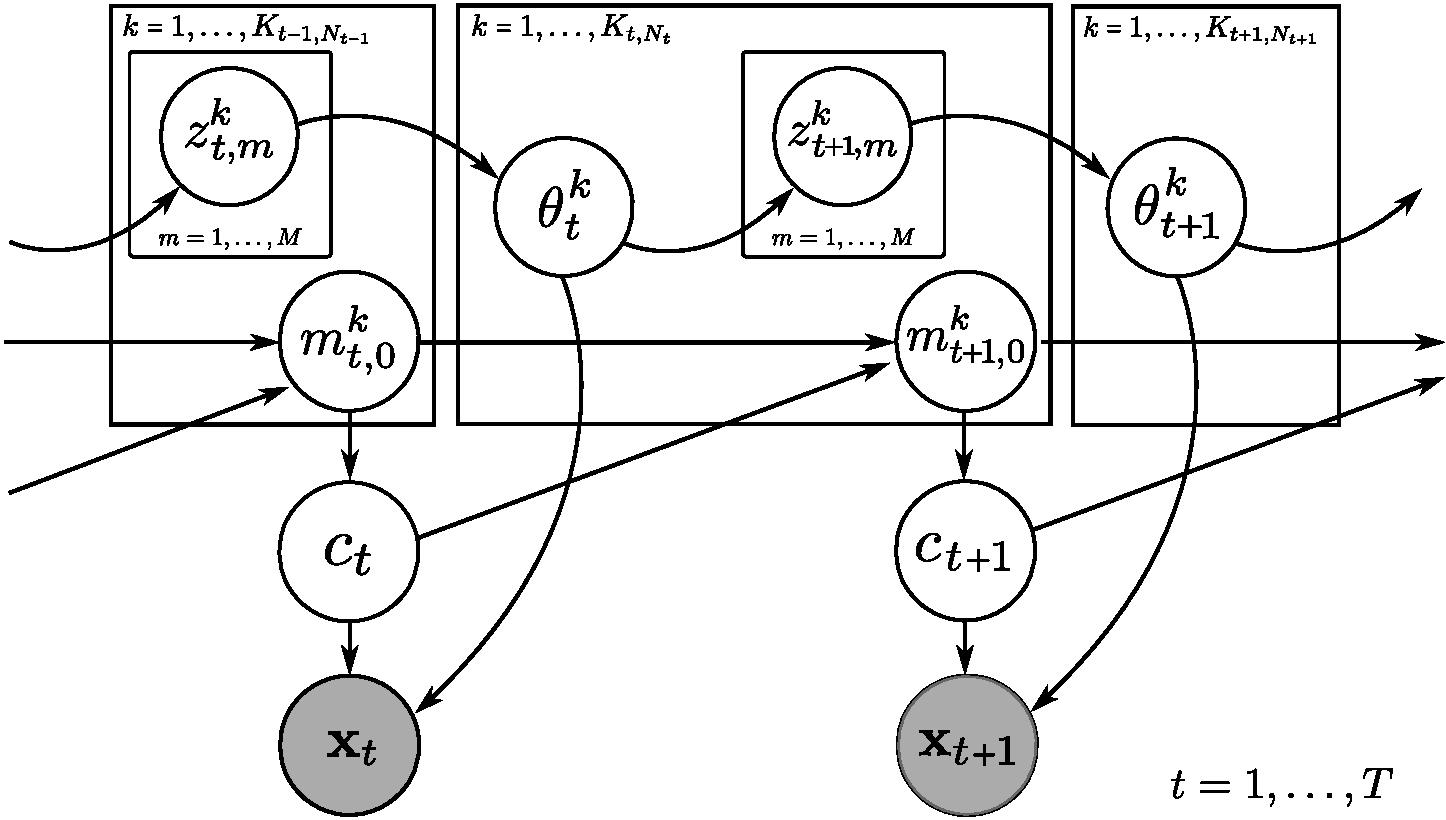
\includegraphics[width=83mm]{ddpmoo_gm.pdf}}
        \caption{\label{fig:gpuddpm_gm_1} Graphical model of the dependent Dirichlet process mixture of objects (DDPMO). All observations at time $t$ are denoted as $\bold{x}_{t}$ and their assignments as $c_{t}$.}
\end{figure}

\subsection{DDPMO}
\label{sec:ddpmoo_def}
The full generative process of the DDPMO is
\begin{enumerate}
    \item At time t=1
    \begin{enumerate}
        \item Draw $\{ c_{1,1:N_1}$, $K_{1,N_1} \}$ $\sim \text{GPU($t=1$)}$
        \item For $k=1,\ldots,K_{1,N_1}$
        \begin{enumerate}
            \item Draw $\theta_1^k \sim \mathbb{G}_0(\boldsymbol{\mu}_0,\kappa_0,\nu_0,\Lambda_0,q_0)$
        \end{enumerate}
        \item For $n=1,\ldots,N_1$
        \begin{enumerate}
            \item Draw $\mathbf{x}_{1,n} \sim \text{F}(\theta_1^{c_{1,n}})$
        \end{enumerate}
    \end{enumerate}
    \item At time $t \geq 2$
    \begin{enumerate}
        \item Draw $\{ c_{t,1:N_t}$, $K_{t,N_t}$, $m_{t,0}^{1:K_{t-1,N_{t-1}}} \}$ $\sim \text{GPU($t \geq 2$)}$
        \item For $k=1,\ldots,K_{t,N_t}$
        \begin{enumerate}
            \item Draw \\$\theta_t^k \sim
                \begin{cases}
                    \text{T}(\theta_{t-1}^k) \hspace{1mm} \text{if} \hspace{1mm} k \leq K_{t-1,N_{t-1}} \\
                    \mathbb{G}_0(\boldsymbol{\mu}_0,\kappa_0,\nu_0,\Lambda_0,q_0) \hspace{1mm} \text{if} \hspace{1mm} k > K_{t-1,N_{t-1}}
                \end{cases}$
        \end{enumerate}
        \item For $n=1,\ldots,N_t$
        \begin{enumerate}
            \item Draw $\mathbf{x}_{t,n} \sim \text{F}(\theta_t^{c_{t,n}})$
        \end{enumerate}
    \end{enumerate}
\end{enumerate}

where the notation $c_{1,1:N_1} = \{ c_{1,1}, \ldots, c_{1,N_1} \}$. A graphical model for the DDPMO is shown in Figure~\ref{fig:gpuddpm_gm_1}.

\section{Inference}
We describe two inference algorithms for the DDPMO: sequential Monte Carlo (SMC) with local Gibbs iterations, and Particle Markov Chain Monte Carlo (PMCMC).

\subsection{Sequential Monte Carlo}
We first derive an SMC (particle filter) inference algorithm where we draw samples from a proposal distribution by iterating through local Gibbs updates (detailed in Section~\ref{sec:localGibbsUpdate}). SMC allows us to make a single pass through the data and draw posterior samples in an online fashion.
\begin{algorithm}[H]
    \caption{SMC for the DDPMO}
    \label{alg:SMC}
    \begin{algorithmic}[1]
        \REQUIRE Extracted pixel data $\{ \mathbf{x}_{1,1:N_1},\ldots,\mathbf{x}_{T,1:N_T} \}$, 
            number of particles $L$, 
            number of local Gibbs iterations $S$
            %, and prior parameters $\alpha$, $\rho$, $\boldsymbol{\mu}_0$, $\kappa_0$, $\nu_0$, $\Lambda_0$ and $q_0$.
        \ENSURE Posterior samples $\left\{\theta_1^{1:K_{1,N_1}},\ldots,\theta_T^{1:K_{T,N_T}}\right\}^{(1:L)}$ 
            of the object model parameters
        \FOR{$t = 1$ {\bfseries to} $T$}
            \FOR{$l = 1$ {\bfseries to} $L$}
                \FOR{iter $= 1$ {\bfseries to} $S$}
                    \STATE Sample $(c_{t,1:N_t})^{(l)} \sim Q_1$ and 
                    $(\theta_t^{1:K_{t,N_t}})^{(l)}$ $\sim$ $Q_2$ 
                \ENDFOR
                \FOR{$k = 1$ {\bfseries to} $K_{t,N_t}$}
                    \STATE Sample $(\Delta m_t^k)^{(l)}$ $\sim$ $\text{Binom}((m_{t,N_t}^k)^{(l)},\rho)$
                    \STATE Set $(m_{t+1,0}^k)^{(l)} = (m_{t,N_t}^k)^{(l)} - (\Delta m_t^k)^{(l)}$
                    \STATE Sample $(z_{t+1,1:M}^k)^{(l)} \sim T_1((\theta_t^k)^{(l)})$ 
                \ENDFOR
                \STATE Compute particle weight $\tilde{w}_{t}^{(l)}$
            \ENDFOR
            %\STATE Normalize particle weights $w_{t}^{(l)}$ $\leftarrow$ 
                %$\frac{\tilde{w}_{t}^{(l)}}{\sum_{l=1}^{L} \tilde{w}_{t}^{(l)} }$   
            \STATE Normalize particle weights and resample particles
        \ENDFOR
    \end{algorithmic}
\end{algorithm}

\subsubsection{Local Gibbs Updates}
\label{sec:localGibbsUpdate}
We perform Gibbs sampling on the assignments and object parameters (at a given $t$) to draw SMC proposals; this allows for the proposal of well-mixed samples given newly introduced data in a particular frame. For an assignment $c_{t,n}$, we can compute a value proportional to the posterior for each possible assignment value $1,\ldots,K_{t,n}$, and then sample from the resulting categorical distribution (after normalizing). The first proposal distribution $Q_1$ is the probability of an assignment $c_{t,n}$ given current cluster sizes, cluster parameters, and concentration parameter $\alpha$, written
\begin{align}
    \label{smc_proposal_1}
    \begin{split}
        &Q_1\left( c_{t,n} | m_{t,n-1}^{1:K_{t,n-1}},  \theta_t^{1:K_{t,n-1}}, \alpha \right) \propto \\
        &\hspace{14mm}\text{Cat}(m_{t,n-1}^1,\ldots,m_{t,n-1}^{K_{t,n-1}}, \alpha) \\ 
        &\hspace{14mm}\times
            \begin{cases}
                \text{F}(\mathbf{x}_{t,n} | \theta_t^{c_{t,n}}) \hspace{2mm} \text{if} \hspace{2mm} c_{t,n} \leq K_{t,n-1} \\
                \int P(\mathbf{x}_{t,n} | \theta) \mathbb{G}_{0}(\theta)d\theta \hspace{2mm} c_{t,n} > K_{t,n-1}
            \end{cases}
    \end{split}
\end{align}
where we set the number of clusters $K_{t,n}$ and their sizes $m_{t,n}^{1:K_{t,n}}$ appropriately as each $c_{t,n}$ is assigned, and assume $K_{1,0}=0$ for consistency at $t=1$. The integral in the case of a new cluster ($k > K_{t,n-1}$) has an analytic solution
\begin{equation}
    \label{marginal_obs_prob}
    \begin{split}
        \int P(\mathbf{x}_{t,n} | \theta)\mathbb{G}_{0} & (\theta) d\theta = \\
        & t_{\nu_0-1}  \left ( \mathbf{x}_{t,n}^{s}  \hspace{1mm} \big{|} \hspace{1mm} 
            \mu_0, \frac{\Lambda_0(\kappa_0+1)}{\kappa_0(\nu_0-1)} \right ) \\
        & \times \prod_{j=1}^V \frac{ \Gamma(\mathbf{x}_{t,n}^c) }  { \Gamma(q_0)}
            \times \frac{\Gamma(\sum_{j=1}^V q_0) }{\Gamma(\sum_{j=1}^V \bold{x}_{t,n}^c) }
    \end{split}
\end{equation}
where $t_{\nu_0-1}$ denotes the multivariate t-distribution with $\nu_0-1$ degrees of freedom, where we follow the three-value parameterization \cite{gelman2004bayesian},
and $\Gamma$ denotes the gamma function.

The conjugacy of appearance model and transition kernel allow us to sample from the second proposal distribution $Q_2$, which is the posterior distribution over the object parameters given current observations, auxiliary variables, and previous time object parameters, written
\begin{align}
    \label{smc_proposal_2}
    \begin{split}
        Q_2(\theta_t^k | \theta_{t-1}^k,\mathbf{x}_{t,1:N_t}^k,&z_{t,1:M}^k) = \\
            &\hspace{1mm} \text{F}(\mathbf{x}_{t,1:N_t}^k | \theta_t^k) 
                %P(z_{t+1,1:M}^k | \theta_t^k) \\
            %&\times P(\theta_t^k | z_{t,1:M}^k) \\
                T_2(\theta_t^k | z_{t,1:M}^k) \\
            &= \hspace{1mm} \text{NiW}(\mu_t^k, \Sigma_t^k | \mu_N, \kappa_N, \nu_N, \Lambda_N) \\
            &\times \text{Dir}( \delta_t^k | q_N)
    \end{split}
\end{align}
where $\mathbf{x}_{t,1:N_t}^k = \{ x_{t,n} \in x_{t,1:N_t} | c_{t,n}=k \} $ and the parameters for the NiW and Dir distributions are given when $\bold{x}_{t,1:N_{t}}^k$ and $z_{t,1:M}^k$ are taken to be the ``observations'' in the following Bayesian updates
\begin{eqnarray}
\label{bayesian_update_1}
    \kappa_N &=& \kappa_0 + N \\
\label{bayesian_update_2}
    \nu_N &=& \nu_0 + N \\
\label{bayesian_update_3}
    \mu_N &=& \frac{\kappa_0}{\kappa_0+N} \mu_0  +  \frac{N}{\kappa_0+N} \overline{\mathbf{x}}^{s}\\
\label{bayesian_update_4}
    \Lambda_N &=& \Lambda_0 + S_{\mathbf{x}^s}\\
\label{bayesian_update_5}
    q_N &=& q_0 + \sum_{i=1}^N \mathbf{x}_i^c
\end{eqnarray}
where $N$ is the number of observations, $\{ \mu_0, \kappa_0, \nu_0, \Lambda_0 \}$ are the NiW prior parameters, $q_0$ is the Dir prior parameter, $\mathbf{x}^s$ and $\mathbf{x}^c$ respectively denote the spatial and color features of the observations, and $\overline{\mathbf{x}}$ and $S_{\mathbf{x}}$ respectively denote the sample mean and sample covariance of the observations.

%Finally, each auxiliary variables $z_{t,m}^k$ can be sampled with
%\begin{equation}
    %z_{t,m}^k \sim \text{Normal}(\mu_{t-1}^k,\Sigma_{t-1}^k)\text{Mult}(\delta_{t-1}^k) 
%\end{equation}

\subsubsection{Particle Weights}
At each time, the particle weights are set to be
\small
\begin{equation}
    \begin{split}
        &\tilde{w}_{t}^{(l)} = \\
            &\frac{ P\left( (c_{t,1:N_t})^{(l)}, (\theta_t^{1:K_{t,N_t}})^{(l)}, \mathbf{x}_{t,1:N_t} | 
                  (\theta_{t-1}^{1:K_{t-1,N_{t-1}}})^{(l)}, (m_{t,0}^{1:K_{t-1,N_{t-1}}})^{(l)}\right) }
                { P\left((c_{t,1:N_t})^{(l)}, (\theta_t^{1:K_{t,N_t}})^{(l)} | 
                  (\theta_{t-1}^{1:K_{t-1,N_{t-1}}})^{(l)}, (m_{t,0}^{1:K_{t-1,N_{t-1}}})^{(l)}\right) }\\
    \end{split}
    \raisetag{60pt}
\end{equation}
\normalsize
where the numerator decomposes into
\small
\begin{equation}
    \begin{split}
        &P\left(\mathbf{x}_{t,1:N_t} | (c_{t,1:N_t})^{(l)}, (\theta_t^{1:K_{t,N_t}})^{(l)} \right)\\
        &\times P\left((c_{t,1:N_t})^{(l)}, (\theta_t^{1:K_{t,N_t}})^{(l)} | 
            (\theta_{t-1}^{1:K_{t-1,N_{t-1}}})^{(l)}, (m_{t,0}^{1:K_{t-1,N_{t-1}}})^{(l)}\right)
    \end{split}
    \raisetag{40pt}
\end{equation}
\normalsize
which can be computed using the DDPMO local probability equations defined in Section~\ref{sec:ddpmoo_def}, and the denominator can be computed using equations \ref{smc_proposal_1} and \ref{smc_proposal_2}.
After the particle weights are computed, they are normalized; particles are then redrawn based on their normalized weights in a multinomial resampling procedure \cite{douc2005comparison}.

\subsubsection{Computational Cost}
Assume $N$ extracted pixels per frame, $T$ frames, $L$ particles, $M$ auxiliary variables, $S$ local Gibbs iterations, and fewer than $K$ sampled objects ($K_{T,N_T}^{(1:L)} \leq K$). In the SMC inference algorithm, each local Gibbs iterations is O$(KN+M)$ and evaluating each particle weight is O$(K+N)$; the SMC algorithm therefore scales as 
%O$(TL(S(KN+M)+KM+K+N))$ $=$ 
O$(TL(K(SN+M)+SM+N))$. If we neglect the number of auxiliary variables $M$, as it is almost always fixed at a small value, the algorithm scales as O$(TLKSN)$.
We have empirically found that an SMC implementation in MATLAB, while not tuned for speed, usually requires 4-20 seconds for every 1 second of video, depending on the number of objects (after frame-rate has been subsampled to approximately 3 images/second in all cases). It is not unreasonable to believe that this could be scaled to real time tracking, given parallel computation  and efficient image processing.
%[Compare with complexity of full-MCMC. In practice, SMC is faster since it yields better results with a smaller number of particles L relative to the number of Gibbs iterations needed for equivalent convergence]

\subsection{Particle Markov Chain Monte Carlo}
SMC provides an efficient, online method for posterior inference, but can suffer from degeneracy; notably, a large majority of the returned particles correspond to a single, non-optimal tracking hypothesis. Ideally, we would like to infer a full posterior over object paths. MCMC methods are guaranteed to yield true posterior samples as the number of samples tends to infinity; however, we have found batch Gibbs sampling to be impractical for inference in the DDPMO, as samples tend to remain stuck in local posterior optima (often when a track begins on one object before switching to another) and cannot converge to a high accuracy tracking hypothesis in a reasonable amount of time.

PMCMC \cite{andrieu2010particle} is a Markov chain Monte Carlo method that attempts to remedy these problems by using SMC as an intermediate sampling step to move efficiently through high dimensional state spaces. We implement a specific case known as the Particle Gibbs (PG) algorithm, where we sample from the conditional distributions used in Gibbs sampling via a modified version of Algorithm 1 referred to as conditional sequential Monte Carlo.

\subsubsection{Conditional SMC}
Conditional SMC \cite{andrieu2010particle} allows for SMC to be used as a proposal distribution in a Gibbs sampling algorithm. We must first introduce the notion of a particle's lineage. 
Let $A_t^{1:L}$ denote the indices of the L particles chosen during the resampling step in time $t$ (in Algorithm 1). The lineage $B_{1:T}^{(l)}$ of a particle is recursively defined as 
$B_T^{(l)} = l$ and for $t=(T-1),\ldots,1$,\hspace{1mm} 
$B_t^{(l)} = A_t^{B_{t+1}^{(l)}}$. More intuitively, for the $l^{th}$ particle, which contains the variables 
$\Theta_{1:T}^{(l)}$ at the final time T, $B_t^{(l)}$ denotes the index of the particle that contained the variables 
$\Theta_{1:t}^{(l)}$$\subset$$\Theta_{1:T}^{(l)}$ at time $t$.

Conditional SMC uses lineages to ensure that a given particle will survive all resampling steps, whereas the remaining particles are generated as before. We define conditional SMC for the DDPMO in Algorithm 2. Note that computation of particle weights and resampling (for relevant particles) is performed in the same manner as in SMC inference (Algorithm 1).
\begin{algorithm}[H]
    \caption{Conditional SMC for the DDPMO}
    \label{alg:SMC}
    \begin{algorithmic}[1]
        \REQUIRE Extracted pixel data $\{ \mathbf{x}_{1,1:N_1},\ldots,\mathbf{x}_{T,1:N_T} \}$, 
            number of particles $L$, 
            number of local Gibbs iterations $S$,
            condition particle $\Phi_{1:T}^{(\eta)}$ with lineage $B_{1:T}^{(\eta)}$ 
            \hspace{1mm}$\left(\eta \in \{ 1,\ldots,L \} \right)$
            %, and prior parameters $\alpha$, $\rho$, $\boldsymbol{\mu}_0$, $\kappa_0$, $\nu_0$, $\Lambda_0$ and $q_0$.
            \ENSURE Particle-conditional posterior samples $\left\{ \Theta_{1:T} \right\}^{(1:L)}$ of all latent model variables
            %\ENSURE Particle-conditional posterior samples for all model parameters 
                %$\left\{ \Theta_{1:T}^{1},\ldots,\Theta_{1:T}^{L} \right\}$
        \FOR{$t = 1$ {\bfseries to} $T$}
            \FOR{$l = 1$ {\bfseries to} $L$}
                \IF{$l \neq B_t^{(\eta)}$}
                    \FOR{iter $= 1$ {\bfseries to} $S$}
                        \STATE Sample $(c_{t,1:N_t})^{(l)} \sim Q_1$ and 
                        $(\theta_t^{1:K_{t,N_t}})^{(l)}$ $\sim$ $Q_2$ 
                    \ENDFOR
                    \FOR{$k = 1$ {\bfseries to} $K_{t,N_t}$}
                        \STATE Sample $(\Delta m_t^k)^{(l)}$ $\sim$ $\text{Binom}((m_{t,N_t}^k)^{(l)},\rho)$
                        \STATE Set $(m_{t+1,0}^k)^{(l)} = (m_{t,N_t}^k)^{(l)} - (\Delta m_t^k)^{(l)}$
                        \STATE Sample $(z_{t+1,1:M}^k)^{(l)} \sim T_1((\theta_t^k)^{(l)})$ 
                    \ENDFOR
                    \STATE Set $\Theta_t^{(l)} = 
                        \left\{ (c_{t,1:N_t})^{(l)},(\theta_t^{1:K_{t,N_t}})^{(l)},(m_{t+1,0}^{1:K_{t,N_t}})^{(l)},\right.$\\ 
                        \hspace{15mm} $\left. 
                        (z_{t+1,1:M}^{1:K_{t,N_t}})^{(l)} \right\}$
                \ELSE
                    \STATE Set $\Theta_t^{(l)} = \Phi_t^{(\eta)}$
                    %\STATE Set $\left\{ (c_{t,1:N_t})^{(B_t^{(\eta)})},(\theta_t^{1:K_{t,N_t}})^{(B_t^{(\eta)})}\right.$,\\ 
                        %\hspace{5mm} $\left.(m_{t+1,0}^{1:K_{t,N_t}})^{(B_t^{(\eta)})}, 
                            %(z_{t+1,1:M}^{1:K_{t,N_t}})^{(B_t^{(\eta)})} \right\}$ 
                        %$=$ $\Theta_{1:t}^{(\eta)}$
                \ENDIF
                \STATE Compute particle weight $\tilde{w}_{t}^{(l)}$
            \ENDFOR
            %\STATE Normalize particle weights $w_{t}^{(l)}$ $\leftarrow$ 
                %$\frac{\tilde{w}_{t}^{(l)}}{\sum_{l=1}^{L} \tilde{w}_{t}^{(l)} }$   
            \FOR{$l = 1$ {\bfseries to} $L$}
                \IF{$l \neq B_t^{(\eta)}$}
                    \STATE Normalize weights and resample particles
                \ENDIF
            \ENDFOR
        \ENDFOR
    \end{algorithmic}
\end{algorithm}

\subsubsection{Particle Gibbs}
In the particle Gibbs (PG) algorithm \cite{andrieu2010particle}, the model variables are first initialized, and then conditional SMC (Algorithm 2) is run for a number of iterations. More specifically, at the end of each iteration, a sample is drawn from the set of weighted particles returned by conditional SMC, and this sample is conditioned upon in the next iteration. The PG algorithm for the DDPMO is formalized in Algorithm 3.

As the PG inference requires all variables to be initialized, SMC inference (Algorithm 1) can be used as a quick way to provide near-MAP initialization of variables.

\begin{algorithm}[h]
   \caption{PMCMC (Particle Gibbs) for the DDPMO}
   \label{alg:SMC}
   \begin{algorithmic}[1]
   \REQUIRE Extracted pixel data $\{ \mathbf{x}_{1,1:N_1},\ldots,\mathbf{x}_{T,1:N_T} \}$, 
        number of global Gibbs iterations $G$,
        number of particles $L$, 
        number of local Gibbs iterations $S$
        %, and prior parameters $\alpha$, $\rho$, $\boldsymbol{\mu}_0$, $\kappa_0$, $\nu_0$, $\Lambda_0$ and $q_0$.
    \ENSURE Posterior samples $\left\{\theta_1^{1:K_{1,N_1}},\ldots,\theta_T^{1:K_{T,N_T}}\right\}^{1:G}$
        of the object model parameters
        \STATE Initialize all model variables to $\Phi_0^{(L)}$
    \FOR{$g=1$ {\bfseries to} $G$}
        \STATE Run conditional SMC (Algorithm 2) with input $\{ \mathbf{x}_{1,1:N_1},\ldots,\mathbf{x}_{T,1:N_T} \}$, 
            $L$, $S$, and conditional on particle $\Phi_{g-1}^{(L)}$ to get particle set 
                $\{\Theta_{1:T}^{(1)},\ldots,\Theta_{1:T}^{(L)}\}$
        \STATE Draw $\Phi_g^{(L)} \sim \text{Unif}(\{\Theta_{1:T}^{(1)},\ldots,\Theta_{1:T}^{(L)}\})$
    \ENDFOR
    \STATE Return $\left\{\theta_1^{1:K_{1,N_1}},\ldots,\theta_T^{1:K_{T,N_T}}\right\}^{1:G}$
        $\in$ $\Phi_{1:G}^{(L)}$
    \end{algorithmic}
\end{algorithm}


\section{Experiments} 
The multivariate Gaussian components of the inferred object model parameters are used to provide centroid sequences (tracks), approximate ovals, and bounding boxes for the objects found in a video.

We first demonstrate the DDPMO on synthetic videos in order to illustrate its ability to track objects through occlusion and infer models of diverse objects. We then apply this model to three true videos to demonstrate finding and tracking objects in difficult detection scenarios, detecting a large number of objects, and using the unsupervised results to automatically train a supervised object detector. We also show how our results compare against detector-based methods on a recent human-tracking benchmark video.


\subsection{Synthetic Videos}

\subsubsection{Tracking through Occlusion}
We first construct simple synthetic videos to demonstrate tracking objects through occlusion (via the learned object models). The first three synthetic videos are each 200 frames and contain a number of colored squares of different (and potentially time-varying) sizes moving at varied speeds and trajectories over a black background. The synthetic videos contain instances of occlusion (of one or more squares) and objects with time-varying appearances, as these notoriously decrease the accuracy of detection and tracking.

The first two videos contain a red and a blue square, which begin at opposite sides of the scene at frame $f=1$ and occlude (blue over red) in the center of the frame at $f=100$ (Figure 3(a)). In the first video, both squares then continue in the same direction, and in the second they reverse directions and end at their initial starting positions. Data extraction yields identical spatial features in both videos; hence, successful tracking depends fully on the model of object color. The third video is the same as the first, except a third green square is added (Figure 3(b)). This square is 50 pixels/side at $f=1$, travels across the frame while linearly shrinking to 10 pixels/side at $f=100$ (where it is occluded), and grows back to 50 pixels/side to end at the opposite side of the frame.

The DDPMO successfully tracked the squares via the SMC inference algorithm in all three occlusion scenarios and correctly modeled the time-varying square in the third video (Figure 4 (a)-(c)).

\subsubsection{Learning Diverse Object Models}
In this experiment, we constructed a video from images of four physically different objects (in shape, scale, and appearance)---a truck, human, cat, and beetle---which randomly walk around the scene. The DDPMO fully tracks all four objects, and accurately learns a diverse set of object models. Inferred results for each object are shown in Figure~4(d)-(g).

\begin{figure}[h!tbp]
        \center{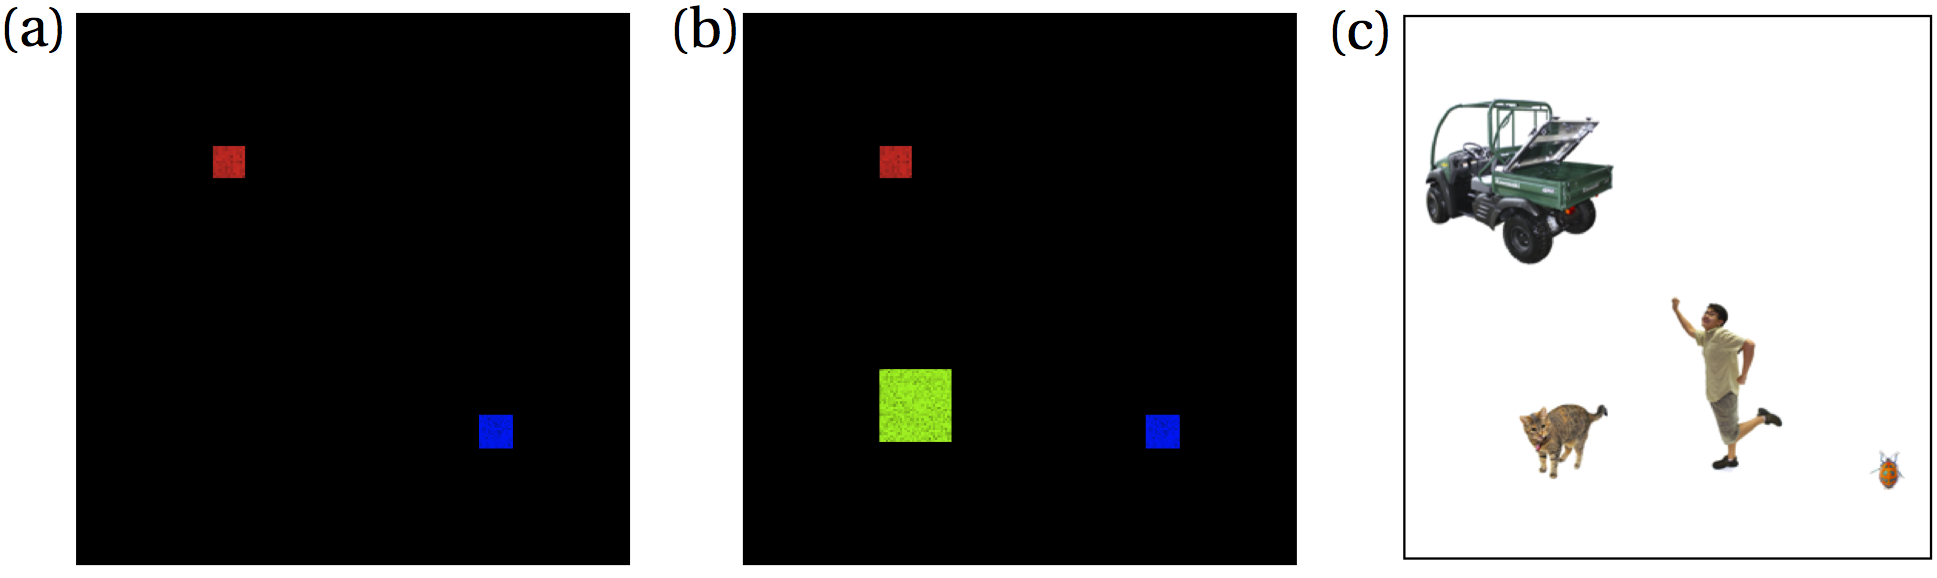
\includegraphics[width=65mm]{synthStillFrame.png}}
        \caption{\label{fig:synthVidFig} Still video frames from synthetic experiments 1 and 2 (a), 3 (b), and 4 (c).}
\end{figure}


\begin{figure}[h!tbp]
        \center{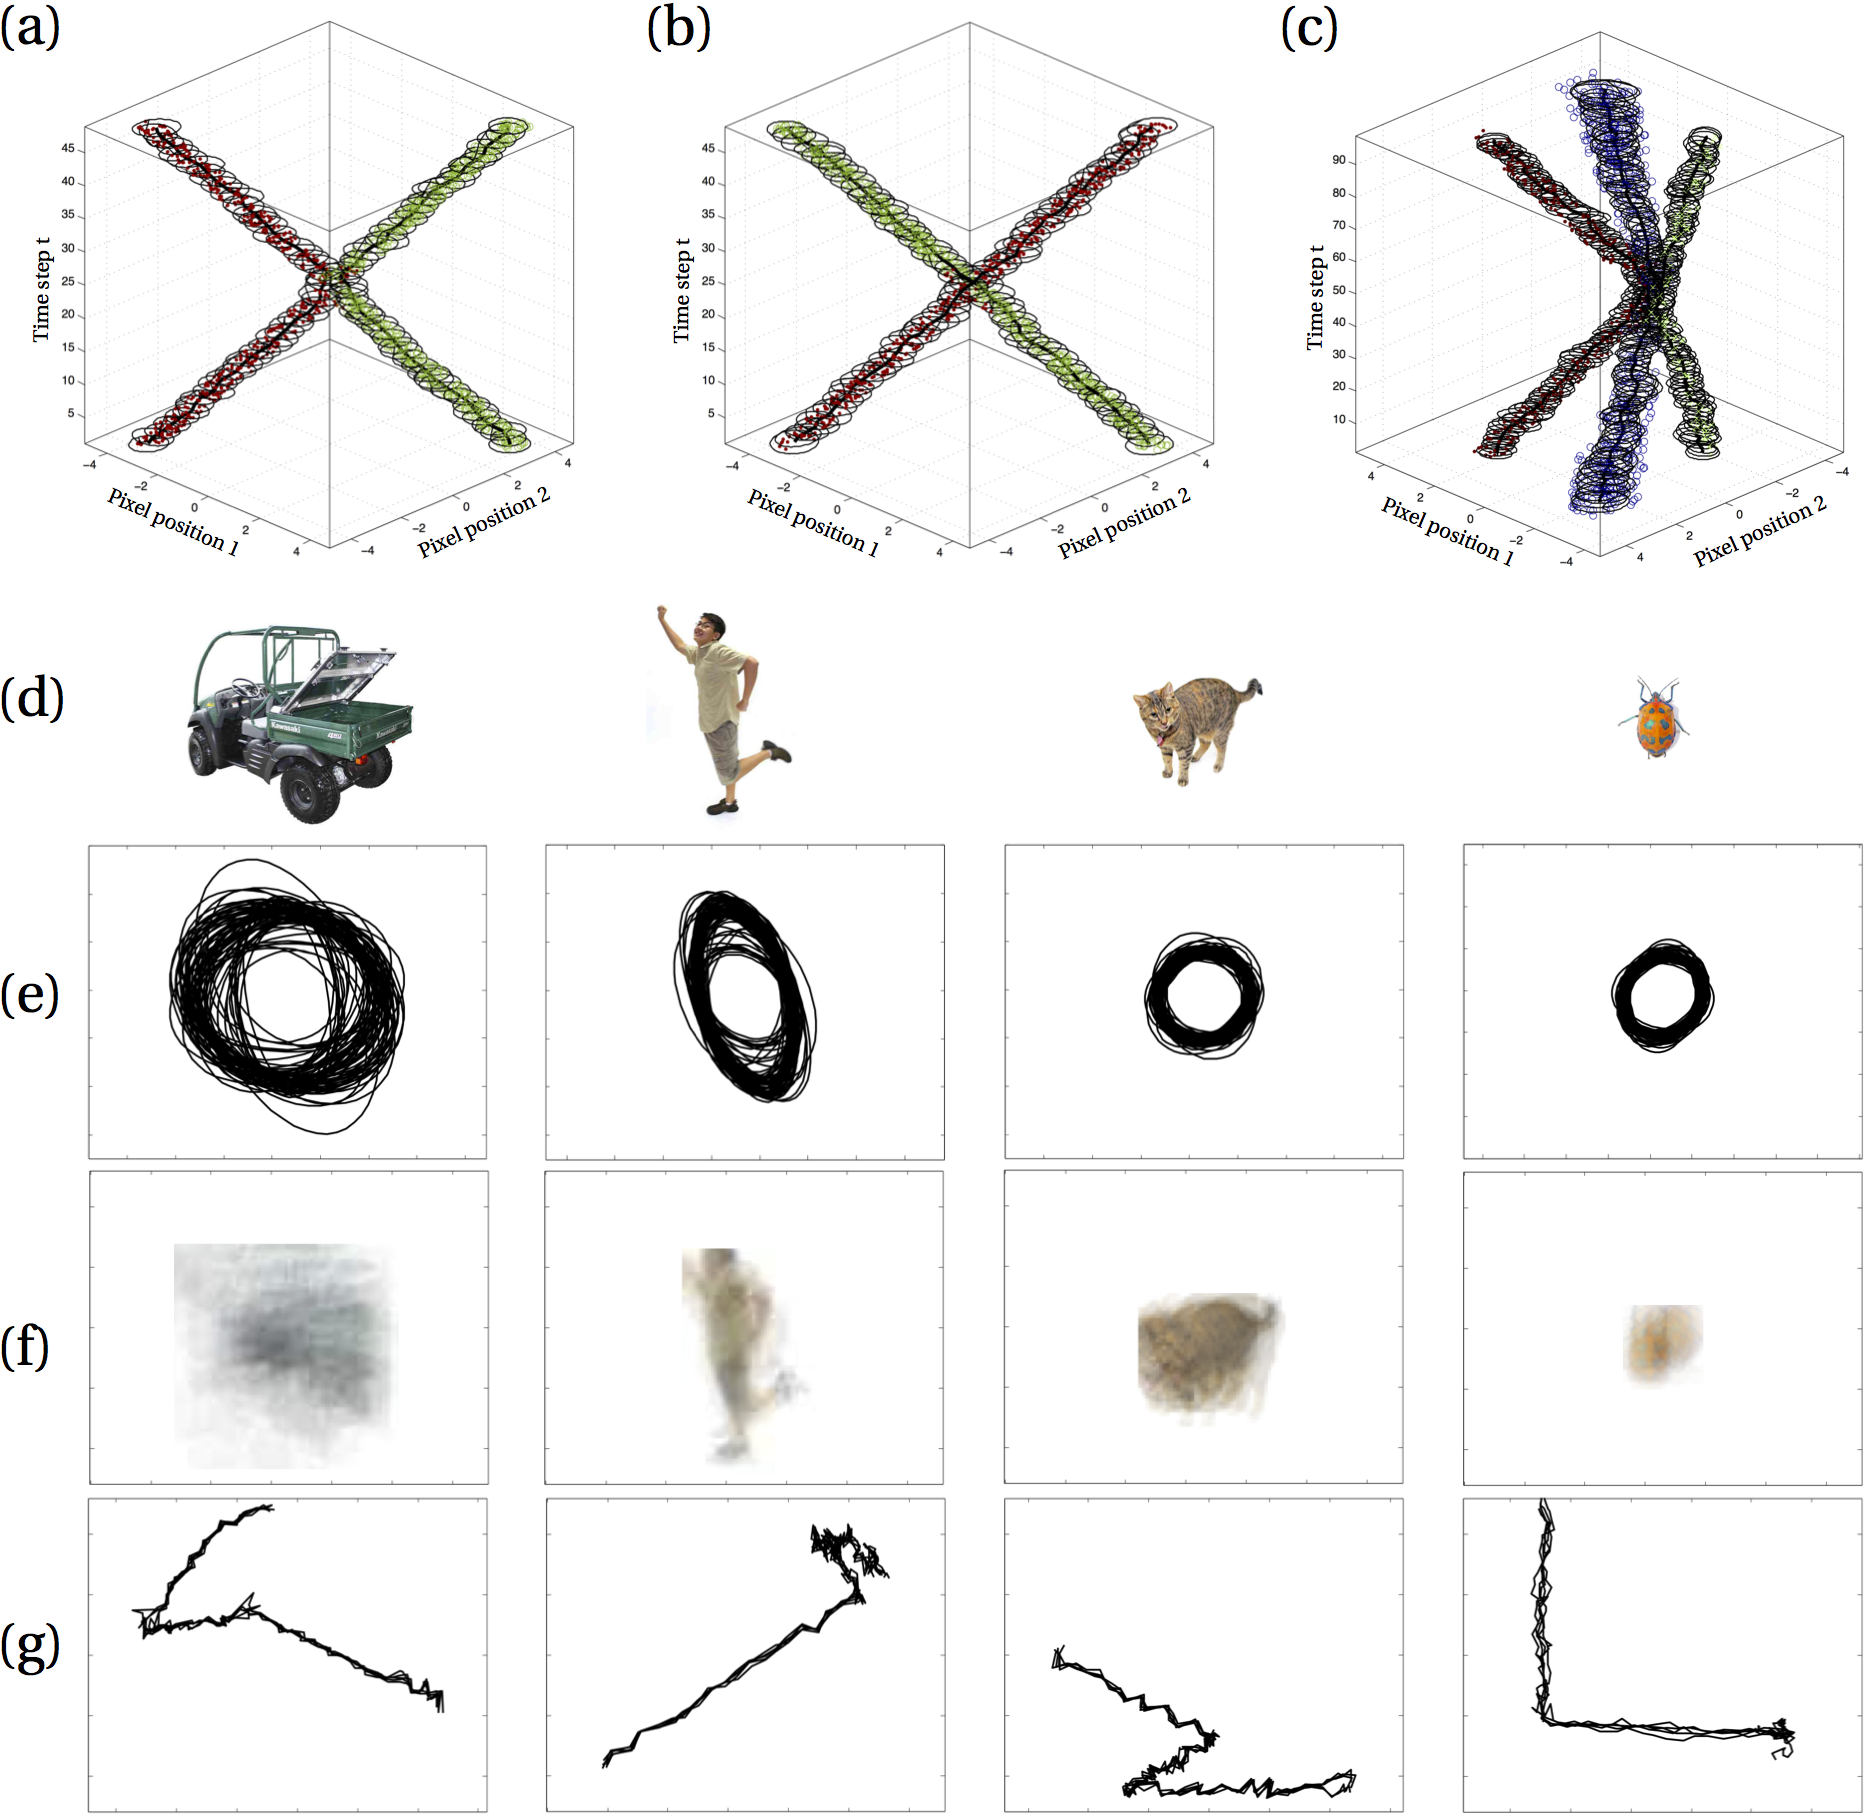
\includegraphics[width=85mm]{synthVidFig.png}}
        \caption{\label{fig:synthVidFig} Inference results are plotted for synthetic experiments 1-3 (a-c). We show the four objects in synthetic experiment 4 (d), samples from the posterior over their spatial parameters (e), averages over extracted color observations for each inferred object (f), and samples from the posterior over the objects' tracks (g).}
\end{figure}

\subsection{Ants Video}
In this experiment, we aim to demonstrate the ability of the DDPMO to find and track objects in a difficult detection scenario. The video contains six ants with a similar texture and color distribution as the background. The ants are hard to discern (even for the human authors), and it is unclear how a predefined detection criteria might be constructed. Futher, the ants move erratically and the spatial data extracted per ant via frame differencing is inconsistent between frames, making it difficult to attempt a simple detection-free tracking method involving independent per-frame segmentation. A still image from the video, with ant locations shown, is given in Figure 5(a).

We compare SMC with PMCMC on this dataset, and find that PMCMC yields more accurate posterior samples (Figure 5(d)) than SMC (5(c)), and infers a more accurate posterior distribution over the number of objects (the posterior on a single frame for both methods is shown in 5(b)).
\begin{figure}[h!tbp]
        \center{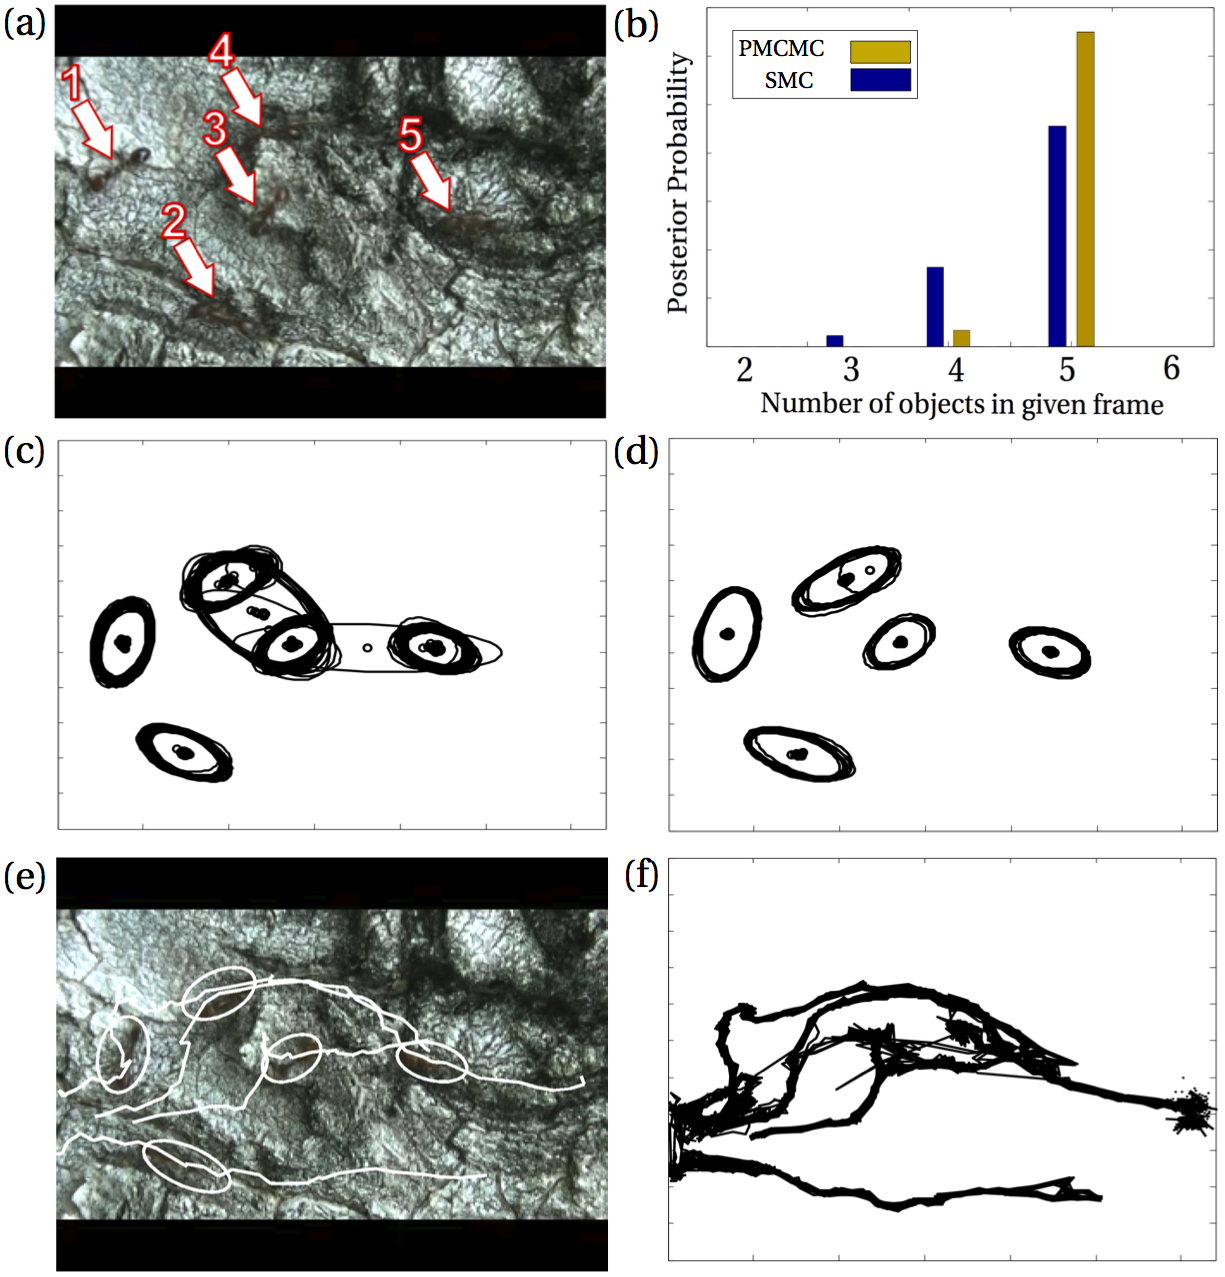
\includegraphics[width=80mm]{antsFig.png}}
        \caption{\label{fig:antsFig} Ants in (a) are difficult to discern (positions labeled). We plot 100 samples from the inferred posterior over object parameters (using SMC (c) and PMCMC (d)) and over object tracks (f). PMCMC proves to give more accurate object parameter samples, which can also be seen by graphing the posterior distribution over the number of objects in the frame (b).}
\end{figure}

\begin{figure}[h!tbp]
        \center{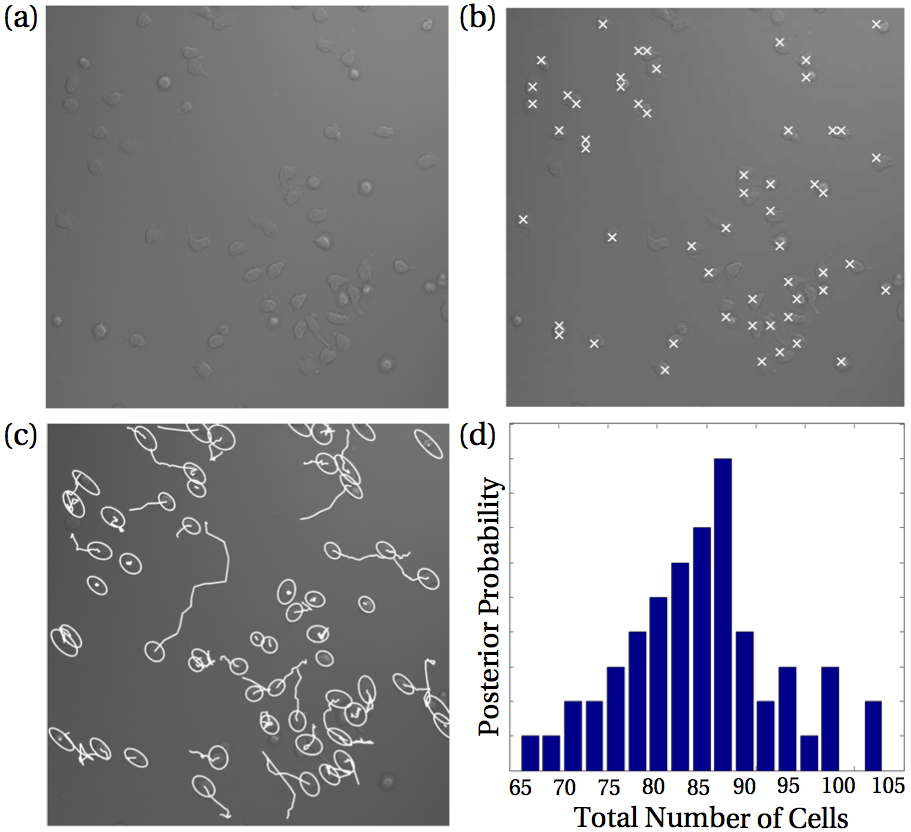
\includegraphics[width=80mm]{tcellFig.png}}
        \caption{\label{fig:antsFig} T cells are numerous, and hard to detect due to low contrast images (a). Inferred detection and tracking results are overlaid in (c). The posterior over number of cells is shown in (d), which peaks near the true value of 92 cells. Inferred cell positions (unsupervised) were used to automatically train an SVM for supervised cell detection; SVM detected positions are shown in~(b).}
\end{figure}

\subsection{T Cells Video}
Automated tracking tools for cells are useful for cell biologist and immunologists studying cell behavior. We present results on a video containing T cells that are hard to detect using conventional methods due to their low constrast appearance against a background (Figure 6(a)). Furthermore, there are a large number of cells (roughly 60 per frame, 92 total). In this experiment, we aim to demonstrate the ability of the DDPMO to perform a tough detection task while scaling up to large numbers of objects. Inference results are shown in Figure 6(c-d).

Futhermore, manually hand-labeling cell positions to train a detector is feasible but time consuming; we show how unsupervised detection results from the DDPMO can be used to automatically train a supervised cell detector (a linear SVM), which can then be applied (via a sliding window across each frame) as a secondary, speedy method of detection (Figure 6(b)).

\subsection{Comparison with Detector-based Methods}
Benchmark video datasets have been produced to provide standard scenes on which researchers can compare detection and tracking results. These videos have been primarily made for surveillance-related workshops, and notably for the International Workshop on Performance Evaluation of Tracking and Surveillance (PETS).

A video dataset used in the PETS2009-2013 conferences (referred to here as PETS2010) was chosen for experimentation due to its prominence in a number of studies (Table 1).
%\cite{ellis_2010,arsic2009multi,berclaz2009multiple,conte2010performance,bolme2009simple,breitenstein2009markovian,ge2009evaluation,alahi2009sparsity,yang2009probabilistic}. 
This video consists of a monocular, stationary camera, 794 frame video sequence containing a number of walking humans. Due to the large number of frames and objects in this video, the SMC inference algorithm was used.

For comparison,  we report two commonly used performance metrics for object detection and tracking, known as the sequence frame detection accuracy (SFDA) and average tracking accuracy (ATA) \cite{kasturi_2008}. These metrics compare detection and tracking results against human-authored ground-truth, where SFDA$\in [0,1]$ corresponds to detection performance and ATA$\in[0,1]$ corresponds to tracking performance. We authored all ground-truth with the Video Performance Evaluation Resource (ViPER) tool \cite{doermann_2000}.

%Parameters for the model were chosen to be $\alpha = 0.1, \rho = 0.8, M = 10, \boldsymbol{\mu}_{0} = (0,0), \kappa_{0} = 0.05, \nu_{0} = 6, \Lambda_{0} = \left( \begin{smallmatrix} 1&0\\ 0&1 \end{smallmatrix} \right), \text{ and } q_{0} = (3, \ldots, 3)$.

\begin{table}
    \begin{tabular}[h!] {| l | l | l |}
        \hline
        \textsc{Method Name} & \textsc{SFDA}  & \textsc{ATA} \\ \hline \hline
        Breitenstein \cite{breitenstein2009markovian} & $ 0.57 $ & $0.30$ \\ \hline
        Yang \cite{yang2009probabilistic} & $ 0.55 $ & $0.45$ \\ \hline
        Conte \cite{conte2010performance} & $ 0.53  $ & $0.06$ \\ \hline
        \textbf{DDPMO} & $ \bold{0.51} $ & $\bold{0.30}$ \\ \hline
        Berclaz \cite{berclaz2009multiple} & $ 0.48 $ & $0.15$ \\ \hline
        Alahi 1 \cite{alahi2009sparsity} & $ 0.43 $ & $0.04$ \\ \hline
        Alahi 2 \cite{alahi2009sparsity} & $ 0.42 $ & $0.05$ \\ \hline
        Bolme 1 \cite{bolme2009simple} & $ 0.41 $ & NA \\ \hline
        Ge \cite{ge2009evaluation} & $ 0.38 $ & $0.04$ \\ \hline
        Bolme 2 \cite{bolme2009simple} & $ 0.34 $ & NA \\ \hline
        Arsic \cite{arsic2009multi} & $ 0.18 $ & $0.02$ \\
        \hline
    \end{tabular}
        \caption{SFDA and ATA performance metric results for the DDPMO and ten human-specific detection-based tracking algorithms on the PETS2010 benchmark dataset. Results are listed in descending order of the SFDA value. The DDPMO performs detection-free tracking of arbitrary objects with comparable accuracy to these human-specific methods. Results provided by the authors of \cite{ellis_2010}.}
        \label{benchmark_results_table}
\end{table}

In Figure 7(a-d), the MAP sample from the posterior distribution over the object parameters is overlayed on the extracted data over a sequence of frames. Figure 7(e) shows the first 50 frames from the video, where the assignment of each data point is represented by color and marker type. The DDPMO is compared against ten state of the art detector-based methods from the PETS2010 conference, and yields comparable results (Figure 7(f)), receiving the fourth highest SFDA score out of eleven, and second highest (tied) ATA score out of 9 (Table 1).
\begin{figure}[h!tbp]
        \center{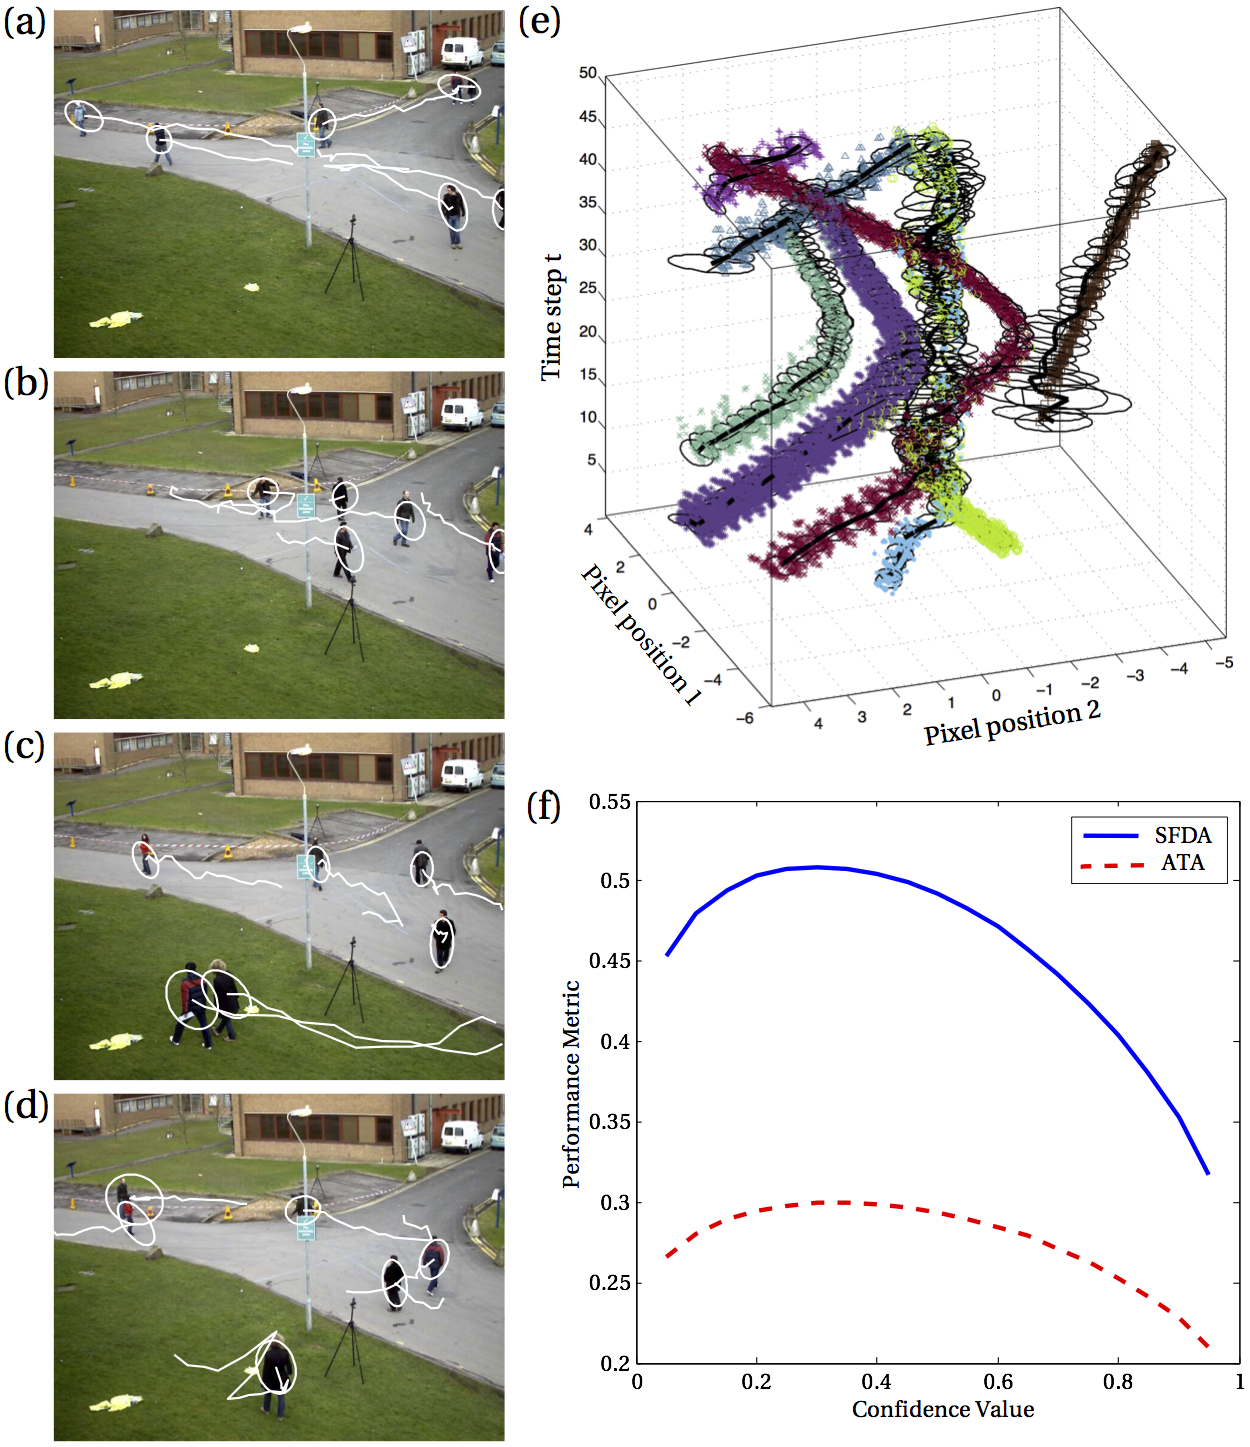
\includegraphics[width=85mm]{pets2009Fig.png}}
        \caption{\label{fig:pets2009Fig} The PETS2010 human tracking benchmark for comparison with object-detector-based methods. MAP object parameter samples are overlaid on still video frames (a-d), and shown along with spatial observations for the first 50 frames (e) (where object assignment variables $c_{t,n}$ are denoted by marker type and color). We plot SFDA and ATA curves over different covariance matrix confidence thresholds~(f), which dictate bounding box width. }
\end{figure}

\vspace{-2mm}
\section{Conclusion}
The DDPMO provides the ability to find, track, and learn a representation for arbitrary objects in video, in a single model framework, to accomplish accurate detection-free tracking.
We detail SMC and PMCMC algorithms for efficient inference and provide results on a number of synthetic and real video datasets that show the ability to track through occlusion, learn models for diverse objects whose appearances may drift, localize objects in difficult detection scenarios, scale to track large numbers of objects, and track certain detectable objects with performance comparable to state of the art detector-based methods.


\begin{small}
\bibliography{ddpTracking_icml}
\bibliographystyle{icml2013}
\end{small}

\end{document}
